\documentclass[aspectratio=169,professionalfonts]{beamer}

\usepackage{hiragino-slides}

\usepackage{marp-beamer-design-flow}

\SetDesign{base}
\SetSlideColor{green}

% これはサンプルです
% 作成者のLT会での発表資料の作成過程に基づきます

\begin{document}

% \TitleFrame{Transformer入門}{ChatGPTの "T" を知る}{坪井 一馬}

{
  \usebackgroundtemplate{%
    
\includegraphics[
      width=\paperwidth,
      height=\paperheight
    ]{drawing.pdf}%
  }
  \setbeamertemplate{footline}{}

  \begin{frame}[plain]
  \end{frame}
}

\TOCFrame

\SectionFrame{自己紹介}{}

\begin{frame}{坪井 一馬}
  \begin{columns}
    \centering
    \begin{column}{0.4\textwidth}
      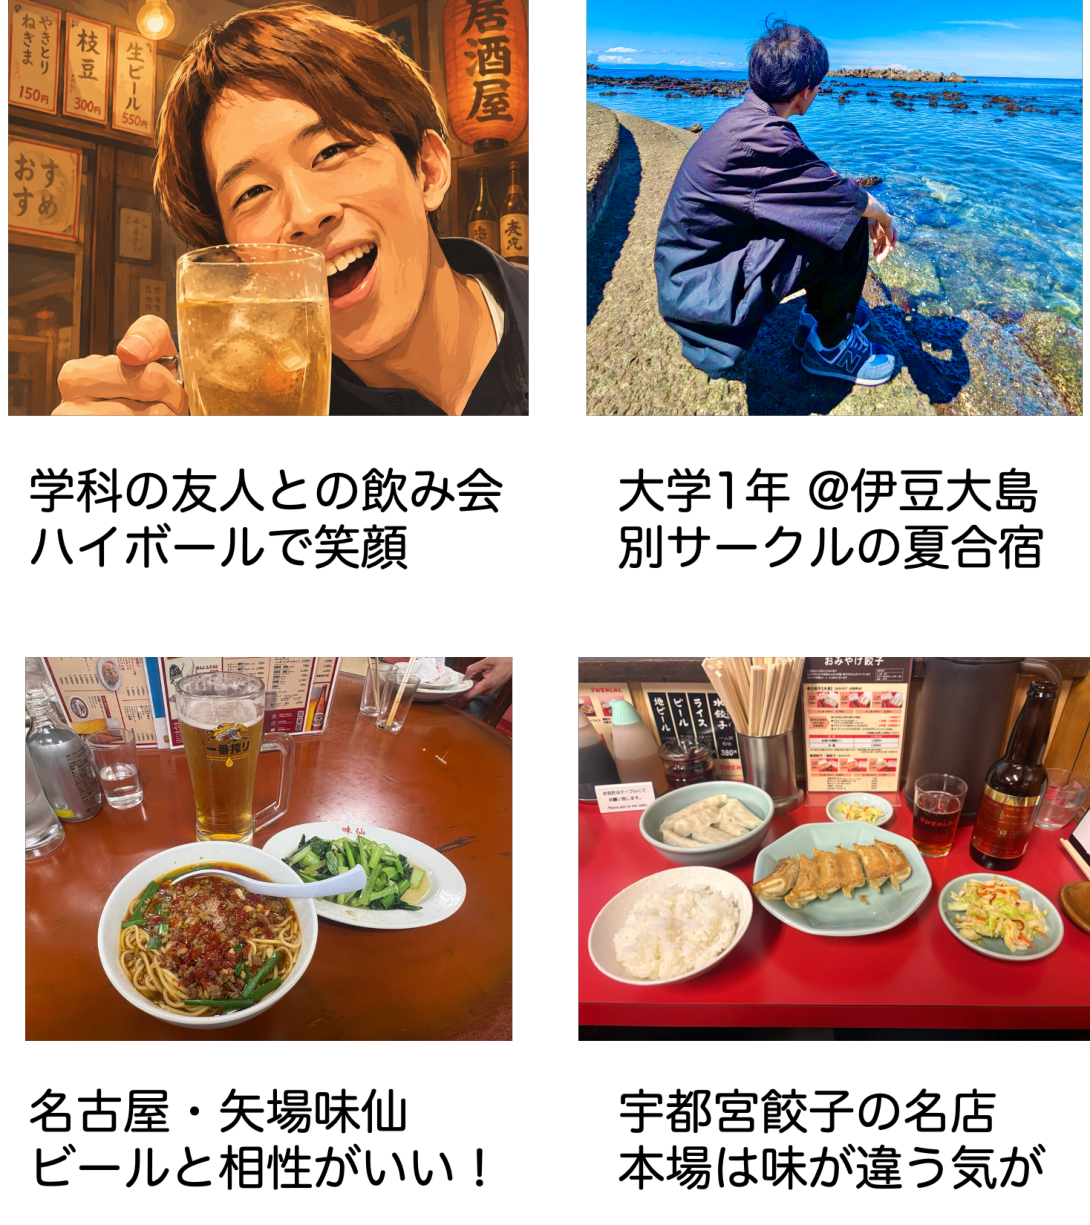
\includegraphics[
      width=\textwidth
    ]{self-introduce.pdf}%
    \end{column}
    \begin{column}{0.4\textwidth}
      \begin{itemize}
        \item \large{\textcolor{red!50!blue}{INTP 論理学者}}
        \item 21歳 神奈川県出身 実家暮らし
        \item 理工学部 化学・生命系学科 化学EP 4年
        \begin{itemize}
          \item 自然言語指示に基づく分子生成モデルを研究しています．
          \item 大学院は内部進学が決まっています．
        \end{itemize}
        \item 東京大学松尾・岩澤研究室の共同研究インターン
        \item Lumosは2年生に加入し，3年生から本格的に活動．
        \begin{itemize}
          \item HP開発等についても中心ではないですが関わっています．
          \item プロジェクトを盛り上げたいという思いで運営に参画．
        \end{itemize}
        \item 以前所属のサークルでケーブルテレビ局の番組制作のリーダーをしていました．
        \item 趣味は様々: 旅行/コーヒー/酒/ゲーム/ラーメン/激辛/ご当地グルメ/名古屋メシ/喫茶店の雰囲気/離島でゆっくり流れる時間を過ごす
      \end{itemize}
    \end{column}
  \end{columns}
\end{frame}


\SectionFrame{Transformerとは何か}{文章を理解する仕組みと，その基本的な考え方を理解する．}

\begin{frame}{Transformerとは何か}
  Transformerとは，文章中の単語同士の関係を捉えるための
  ニューラルネットのアーキテクチャである．

  \begin{itemize}
    \item 2017年に翻訳モデルとして提案されるが，画像生成等にも応用されるようになっている．
    \item Attention機構というメカニズムを中心に据える．
    \item 現在のLLMの基盤技術となっている．
  \end{itemize}
\end{frame}

\SectionFrame{Attentionの考え方}{文脈の中でどの単語に注目するべきかを重要度に基づいて考える．}

\begin{frame}{段組が入るかどうか}
  ちゃんと段組を入れることもできますか？
  
  \begin{columns}
    \centering
    % 左側の列（全体の0.48倍の幅）
    \begin{column}{0.4\textwidth}
      ここに左側の文章や箇条書きを書きます。
      \begin{itemize}
        \item 要素A
        \item 要素B
      \end{itemize}
    \end{column}
    
    % 右側の列（全体の0.48倍の幅）
    \begin{column}{0.4\textwidth}
      ここに右側の画像や文章を書きます。
      %\includegraphics[width=\linewidth]{example-image}
    \end{column}
  \end{columns}
\end{frame}

\begin{frame}{Attentionの考え方}
  以下の例文を理解するとき，どう考えるか？

  \begin{quote}
    私は昨日，\textbf{銀行}に行ってお金を下ろした．
  \end{quote}

  「銀行」を理解するときは，「お金」や「下ろした」との関係に注目します．
\end{frame}

\SectionFrame{Transformerの構造}{入力された文章が処理される流れを整理します．}

\begin{frame}{Transformerの構造}
  入力
  \begin{itemize}
    \item 文章をトークン列として入力する．
  \end{itemize}
\end{frame}

\SectionFrame{Transformerの構造}{入力された文章が処理される流れを整理します．}


\SectionFrame{Transformerの構造}{入力された文章が処理される流れを整理します．}


\SectionFrame{Transformerの構造}{入力された文章が処理される流れを整理します．}


\SummaryFrame{まとめ}{%
  \begin{itemize}
    \item Transformerは単語同士の関係を捉える
    \item Attentionが文脈に応じた重要度を計算する
    \item 現在の大規模言語モデルを支える基盤技術である
  \end{itemize}
}

\end{document}
